\chapterimage{shell.jpg} 
\chapter{SSH}
\label{C:ssh}
\index{ssh}

/FILENAME/

If you do not know what ssh is we recommend that you
\href{http://openssh.com/manual.html}{read up on it}. However, the
simple material presented here will help you get started quickly. It
can however not replace the more comprehensive documentation. We also
remommend that you read this entire section first before you start
past and copy style tutorials as this will not allow you to understand
the way ssh is used. FOr this reason we start with the explanation of
ssh and not the setup on your machine. We want you to obtain first a
solid overview of what you need to do.

To access remote resources this is often achieved via SSH. You need to
provide a public ssh key to FutureSystem. We explain how to generate a
ssh key, upload it to the FutureSystem portal and log onto the
resources. This manual covers UNIX, Mac OS X, as well as Windows 10.



\section{Generate a SSH key}
\label{s:generate-a-ssh-key}
\index{ssh-keygen}

First we must generate a ssh key with the tool
\href{http://linux.die.net/man/1/ssh-keygen}{ssh-keygen}. This program
is commonly available on most UNIX systems (this includes Cygwin if
you installed the ssh module or use our pre-generated cygwin
executable). It will ask you for the location and name of the new
key. It will also ask you for a passphrase, which you \textbf{MUST}
provide. Please use a strong passphrase to protect it
appropriately.

\begin{WARNING}
  Some teachers and teaching assistants advice you to not use
  passphrases. This is \textbf{WRONG} as it allows someone that gains
  access to your computer to also gain access to all resources that
  have the public key.
\end{WARNING}

In case you already have a ssh key in your machine, you can reuse it and
skip this whole section.

To generate the key, please type:

Example:

\begin{verbatim}
ssh-keygen -t rsa -C localname@indiana.edu
\end{verbatim}

This command requires the interaction of the user. The first question
is:

\begin{verbatim}
Enter file in which to save the key (/home/localname/.ssh/id_rsa): 
\end{verbatim}

We recommend using the default location \textasciitilde{}/.ssh/ and the
default name id\_rsa. To do so, just press the enter key.

Your \emph{localname} is the username on your computer.

The second and third question is to protect your ssh key with a
passphrase. This passphrase will protect your key because you need to
type it when you want to use it. Thus, you can either type a passphrase
or press enter to leave it without passphrase. To avoid security
problems, you \textbf{MUST} chose a passphrase. Make sure to not just
type return for an empty passphrase:

\begin{verbatim}
Enter passphrase (empty for no passphrase):
\end{verbatim}

and:

\begin{verbatim}
Enter same passphrase again:
\end{verbatim}

If executed correctly, you will see some output similar to:

\begin{verbatim}
Generating public/private rsa key pair.
Enter file in which to save the key (/home/localname/.ssh/id_rsa): 
Enter passphrase (empty for no passphrase):
Enter same passphrase again:
Your identification has been saved in /home/localname/.ssh/id_rsa.
Your public key has been saved in /home/localname/.ssh/id_rsa.pub.
The key fingerprint is:
34:87:67:ea:c2:49:ee:c2:81:d2:10:84:b1:3e:05:59 localname@indiana.edu

+--[ RSA 2048]----+
|.+...Eo= .       |
| ..=.o + o +o    |
|O.  = ......     |
| = .   . .       |
+-----------------+
\end{verbatim}


Once, you have generated your key, you should have them in the \verb|.ssh|
directory. You can check it by:

\begin{verbatim}
$ cat ~/.ssh/id_rsa.pub
\end{verbatim}

If everything is normal, you will see something like:

\begin{verbatim}
ssh-rsa AAAAB3NzaC1yc2EAAAADAQABAAABAQCXJH2iG2FMHqC6T/U7uB8kt
6KlRh4kUOjgw9sc4Uu+Uwe/kshuispauhfsjhfm,anf6787sjgdkjsgl+EwD0
thkoamyi0VvhTVZhj61pTdhyl1t8hlkoL19JVnVBPP5kIN3wVyNAJjYBrAUNW
4dXKXtmfkXp98T3OW4mxAtTH434MaT+QcPTcxims/hwsUeDAVKZY7UgZhEbiE
xxkejtnRBHTipi0W03W05TOUGRW7EuKf/4ftNVPilCO4DpfY44NFG1xPwHeim
Uk+t9h48pBQj16FrUCp0rS02Pj+4/9dNeS1kmNJu5ZYS8HVRhvuoTXuAY/UVc
ynEPUegkp+qYnR user@myemail.edu
\end{verbatim}

\section{Add or Replace Passphrase}

In case you need to change your change passphrase, you can simply run
\verb|ssh-keygen -p| command. Then specify the location of your current
key, and input (old and) new passphrases. There is no need to
re-generate keys:

\begin{verbatim}
ssh-keygen -p
\end{verbatim}

You will see the following output once you have completed that step:

\begin{verbatim}
Enter file in which the key is (/home/localname/.ssh/id_rsa):
Enter old passphrase:
Key has comment '/home/localname/.ssh/id_rsa'
Enter new passphrase (empty for no passphrase):
Enter same passphrase again:
Your identification has been saved with the new passphrase.  
\end{verbatim}

\section{SSH Add and Agent}
\index{ssh add}

To not always type in your password, you can use \verb|ssh-add|.

It prompts the user for a private key passphrase and add it to a list
of keys managed by the ssh-agent. Once it is in this list, you will
not be asked for the passphrase as long as the agent is running.with your public key.

To start the agent please use the following command:

\begin{verbatim}
eval `ssh-agent`
\end{verbatim}

It is important that you use the backquote (`), located under the
tilde (~), rather than the single quote ('). Once the agent is started
it will print a PID that you can use to interact with later

To add the key use the command

\begin{verbatim}
ssh-add
\end{verbatim}

To remove the agent use the command

\begin{verbatim}
kill $SSH_AGENT_PID
\end{verbatim}

To execute the command upon logout, place it in your 
\verb|.bash_logout| (assuming you use bash).


\section{SSH Config}
\index{ssh config}

\TODO{describe ssh config}

\section{SSH Port Forwarding}
\index{ssh port forwarding}

\TODO{describe port forwarding}

\section{Upload the key to gitlab}\label{upload-the-key-to-gitlab}

\begin{IU}
We do not use gitlab.com for most classes but use github.com
\end{IU}

In case you use gitlab  Follow the instructions provided here to
upload the public key

  \URL{http://docs.gitlab.com/ce/ssh/README.html}

\section{Using SSH on Mac OS X}\label{using-ssh-on-mac-os-x}


Mac OS X comes with an ssh client. In order to use it you need to open
the \texttt{Terminal.app} application. Go to \texttt{Finder}, then click
\texttt{Go} in the menu bar at the top of the screen. Now click
\texttt{Utilities} and then open the \texttt{Terminal} application.


\section{Using SSH on Linux}\label{using-ssh-on-mac-os-x}

All Linux versions come with ssh and can be used right from the terminal.

\section{Using SSH on Raspberry Pi 3}\label{using-ssh-on-mac-os-x}

Install Rasbian on an SD card, and boot up your system. Before putting
it on the network, reset the default user password with the
\verb|passwd| command.Now you can use the terminal and use ssh just
like on any Linux computer.



\section{SSH on Windows}

\begin{WARNING}
For this class we recommend that you use a virtual
machine via virtual box and use the Linux ssh instructions. The
information here is just provided for completness and no support will be
offered for native windows support.
\end{WARNING}

Windows users need to have some special software to be able to use the
SSH commands. If you have one that you are comfortable with and know how
to setup key pairs and access the contents of your public key, please
feel free to use it.

On Windows you have a couple of options on running Linux commands such
as ssh. At this time it may be worth while to try the OpenSSH CLient
available for Windows, although it is in beta. If you like to use
other methods we have included alternatives.

\subsection{OpenSSH Client (Beta)}

\TODO{provide us with screenshots of the  windows.}

In case you need access to ssh Microsoft has furtunately updated their
software to be able to run it directly from the Winodws commandline
including PowerShell.

However it is as far as we know not activated by default so you need
to follow some setup scripts. Also this software is considered beta
and its development and issues can be found at

\URL{https://github.com/PowerShell/Win32-OpenSSH}
\URL{https://github.com/PowerShell/Win32-OpenSSH/issues}

What you have to do is to install it by going to \verb|Settings > Apps|
and click \verb|Manage optional features| under \verb|Apps & features|.

Next, Click on the \verb|Add feature|. You will be presented with a
list in which you scroll down, till you find
\verb|OpenSSH Client (Beta)|. Click on it and invoke \verb|Install|.

After the install has completed, you can use the \verb|ssh| command.
Just type it in the commandshell or PowerShell 

\begin{verbatim}
PS C:\Users\gregor> ssh
\end{verbatim} 

Naturally you can now use it just as on Linux or OSX. and use it to
login to other resources 

\begin{verbatim}
PS C:\Users\gregor> ssh myname@computer.example.com
\end{verbatim} 


\subsection{Using SSH from Cygwin}

One established way of using ssh is from using cygwin.

  \URL{http://cygwin.com/install.html}

Cygwin contains a collection of GNU and Open Source tools providing
Linux like functionality on Windows.  A DLL is available that
exposes the POSIX API functionality.

A list of supported commands is available at 

\URL{https://cygwin.com/packages/package_list.html}

Please be minded that in order for cygwin to function easily the
Windows user name should not include spaces. However, as the setup in
windows encourages to use the full name whne you buy and setup a
machine it may not be convenient to use. However, we just recommend
that you create yourself a new username and use this if you like to
use cygwin.

You can selectively install from the cygwin setup terminal which
software you like to use, obviously you may want to use ssh

\subsection{SSH from putty}\label{S:putty}
\index{putty}

As you will see the process is somewhat cumbersome and when you
compare it with the commandline tools available, we do recommend using
them instead.

PuTTY allows you to access the SSH, Telnet and Rlogin network
protocols from windows. 

\URL{https://www.chiark.greenend.org.uk/~sgtatham/putty/latest.html}

Although PuTTY has been out there for many years and served the
community well, it is not following the standard ssh command line
syntax when invoced from a command shell.

\begin{verbatim}
putty -ssh user@host.name
\end{verbatim}

In addition to using ssh, it also provides a copy command.

\begin{verbatim}
pscp user@host.name:"\"remote filename with spaces\"" local_filename
\end{verbatim}

Putty is best known for its GUI configuration application to manage
several machines as demonstrated next. Once you have downloaded it and
opened PuTTYgen, you will be presented with a a key generator window
(images provided by chameleon cloud) (see Figure~\ref{F:putty-key}).

\FIGURE{htb} 
       {0.5}
       {images/chameleon/putty2.png}
       {Key generation window}
       {F:putty-key} 

To generate a key you click the \textit{Generate} button which is
blue. The PuTTY Key Generator (see Figure~\ref{F:putty-pass})
will then ask you to move your mouse around the program's blank
space to generate ``randomness'' for your key.  You must enter a
``Key passphrase'' and then confirm the passphrase.

\FIGURE{htb} 
       {0.5}
       {images/chameleon/putty3.png}
       {Key generation window}
       {F:putty-pass} 


Next you need to save both the public and private keys into a file of your choice using
the ``Save public key'' and ``Save private key'' buttons. We suggest
you name something obvious like ``public\_key.pub'' and ``private\_key'' so that you
can distinguish between the two.


Before closing this window, select the entire public key and copy it
with ``Control-C''. Please note that everything should be copied,
including ``ssh-rsa''. This will be used when importing the key pair to
Openstack.

At this time, the public key has been created and copied. Now you can
use the public key and upload it to systems you like to ligin to.


\subsection{Chocolatey}
\index{chocolatey}

Another approach is to use it in Powershell with the help of
chopolatey. Other options may be better suited for you and we leave it
up to you to make this decission. 

Chocolatey is a software management tool that mimics the install
experience that you have on Linux and OSX. It has a repository with
many packages. The packages are maintained by the community and you
need to evaluate security implications when installing packages hosted
on chocolatey just as you have to do if you install software on LInux
and OSX from their reporsitories.  Please be aware that there could be
malicious code offered in the chocolatey repository although the
distributors try to remove them.

The installation is sufficently explained at

  \URL{https://chocolatey.org/install}

Once installed you have a command choco and you should make sure you
have the newest version with:

\begin{verbatim}
choco upgrade chocolatey
\end{verbatim}

Now you can browse packages at

\URL{https://chocolatey.org/packages}

Search for openssh and see the results. You may find different versions.
Select the one that most suits you and satisfies your security
requirements as well as your architecture. Lets assume you chose the
Microsoft port, than you can install it with:

\begin{verbatim}
choco install openssh
\end{verbatim}

Naturally, you can also install cygwin and ptty over chocolatey. A
list of packages can be found at 

\URL{https://chocolatey.org/packages}

Packages of interest include

\begin{itemize}

\item emacs: choco install emacs
  \URL{https://chocolatey.org/packages/Emacs}

\item pandoc: choco install pandoc
  \URL{https://chocolatey.org/packages/pandoc}

\item LaTeX: choco install miktex
  \URL{https://chocolatey.org/packages/miktex}

\item jabref: choco install jabref
  \URL{https://chocolatey.org/packages/JabRef}

\item pycharm: choco install pycharm-community
  \URL{https://chocolatey.org/packages/PyCharm-community}

\item lyx: choco install lyx
  \URL{https://chocolatey.org/packages/lyx}

\item python 2: choco install python2
  \URL{https://chocolatey.org/packages/python2}

\item python 3: choco install python
  \URL{https://chocolatey.org/packages/python/3.6.4}

\item pip: choco install pip
  \URL{https://chocolatey.org/packages/pip}

\item virtualbox: choco install virtualbox
  \URL{https://chocolatey.org/packages/virtualbox}

\item vagrant: choco install vagrant
  \URL{https://chocolatey.org/packages/vagrant}

\end{itemize}

Before installing any of them evaluate if you need them and identify
security risks.


\section{Tips}

\begin{description}

\item[Use SSH keys] You will need to use ssh keys to access remote machines

\item[No blank passphrases] In most cases you must use a passphrase
  with your key. In fact if we find that you use passwordless keys to
  futuresystems and to chameleon cloud resources, we may elect to give
  you an \textit{F} for the assignment in question. There are some
  exceptions, but they will be clearly communicated to you in
  class. You will as part of your cloud drivers license test explain
  how you gain access to futuresystmes and chameleon to explicitly
  explain this point and provide us with reasosns what you can not do.

\item[A key for each server] Under no circumstances copy the same
  private key on multiple servers. THis violates security best
  practices. Create for each server a new private key and use their
  public keys to gain access to the appropriate server.

\item[Use SSH agent] So as to not to type in all the time the
  passphrase for a key, we recommend using ssh-agent to manage the
  login. This will be part of your cloud drivers license.

  But shut down the ssh-agent if not in use

\item[keep an offline backup, put encrypt the drive] You may for some
  of our projects need to make backups of private keys on other
  servers you set up. If you  like to make a backup you can do so on a
  USB stick, but make sure that access to the stick is encrypted. Do
  not stor anything else on that key and look it in a safe place. If
  you lose the stick, recreate all keys on all machines.

\end{description}


\section{SSH to FutureSystems Resources}
\index{ssh!Futuresystems}

Next, you need to upload the key to the portal. You must be logged into
the portal to do so.

\begin{description}

\item[Step 1:] Log into the portal \medskip

\begin{center}
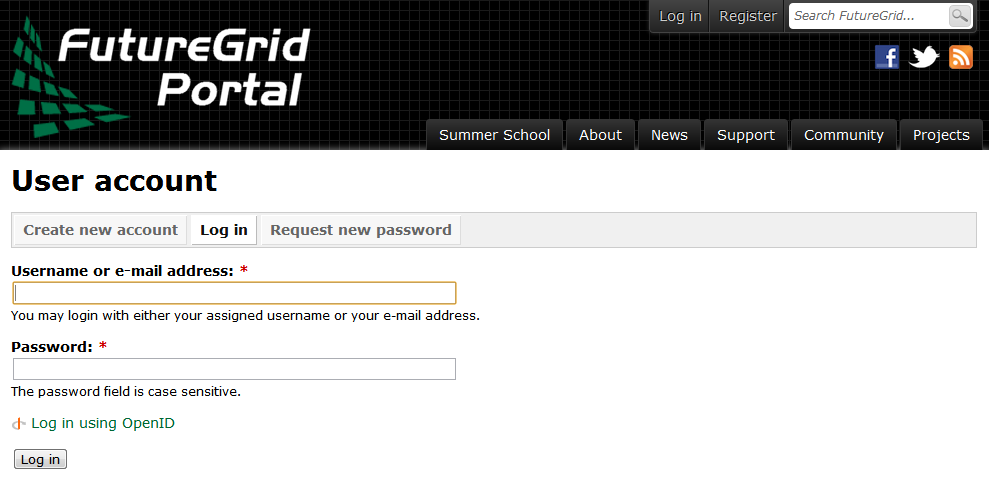
\includegraphics[width=0.5\textwidth]{/images/portalLogin_0.png}
\end{center}

\item[Step 2:] Click in the ``ssh key'' button or go directly to
  \url{https://portal.futuresystems.org/my/ssh-keys} \medskip

\begin{center}
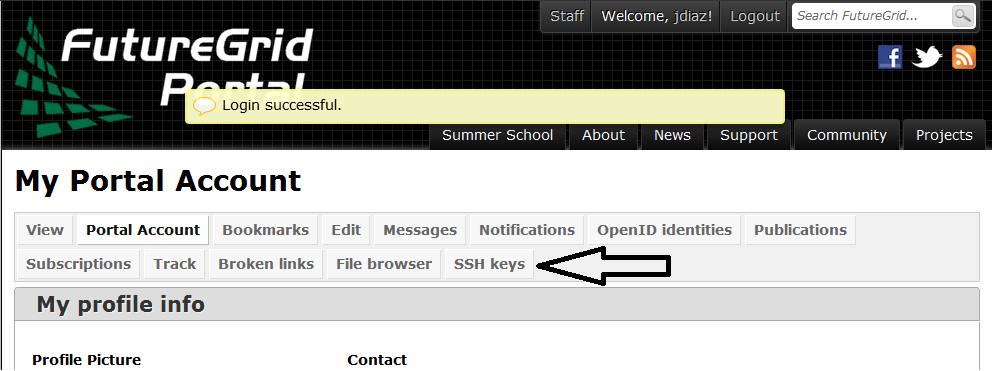
\includegraphics[width=0.5\textwidth]{/images/portalsshkey.png}
\end{center}

\item[Step 3:] Click in the ``add a public key'' link.  \medskip

\begin{center}
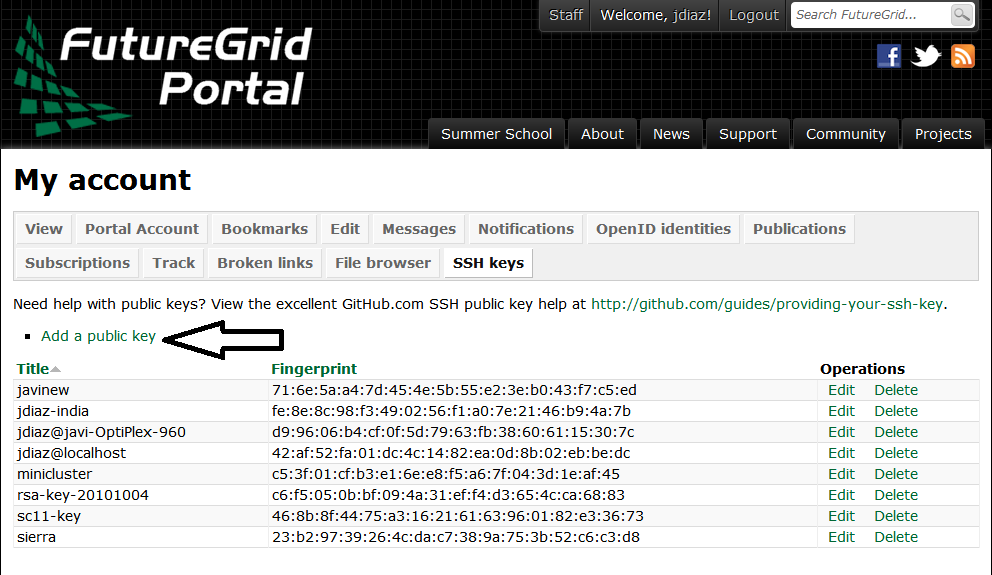
\includegraphics[width=0.5\textwidth]{/images/portalclikaddkey_0.png}
\end{center}

\item[Step 4:] Paste your ssh key into the box marked Key. Use a text
  editor to open the ``id\_rsa.pub''. Copy the entire contents of this
  file into the ssh key field as part of your profile
  information. Many errors are introduced by users in this step as
  they do not paste and copy correctly.  \medskip

\begin{center}
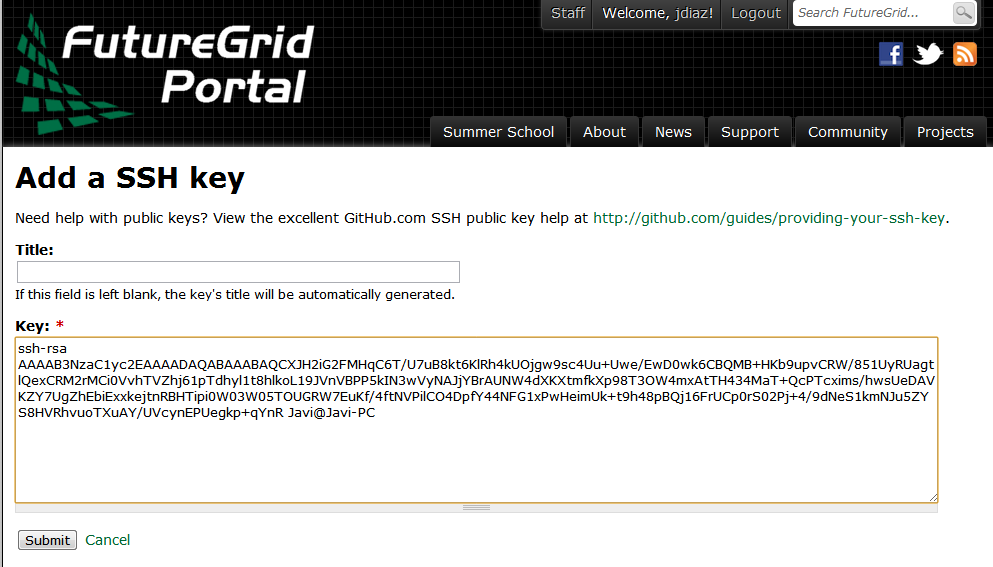
\includegraphics[width=0.5\textwidth]{/images/portalkeypaste_0.png}
\end{center}

\item[Step 5:] Click the submit button. \textbf{IMPORTANT}: Leave the
  Title field blank.  Make sure that when you paste your key, it does
  not contain newlines or carriage returns that may have been
  introduced by incorrect pasting and copying. If so, please remove
  them.

\end{description}

At this point, you have uploaded your key. However, you will still need
to wait till all accounts have been set up to use the key, or if you did
not have an account till it has been created by an administrator.
Please, check your email for further updates. You can also refresh this
page and see if the boxes in your account status information are all
green. Then you can continue.

\section{Testing your ssh key}\label{testing-your-ssh-key}

If you have had no FutureSystem account before, you need to wait for up
to two business days so we can verify your identity and create the
account. So please wait. Otherwise, testing your new key is almost
instantaneous on india. For other clusters like it can take around 30
minutes to update the ssh keys.

To log into india simply type the usual ssh command such as:

\begin{verbatim}
$ ssh portalname@india.futuresystems.org
\end{verbatim}

The first time you ssh into a machine you will see a message like this:

\begin{verbatim}
The authenticity of host 'india.futuresystems.org (192.165.148.5)' can't be established.
RSA key fingerprint is 11:96:de:b7:21:eb:64:92:ab:de:e0:79:f3:fb:86:dd.
Are you sure you want to continue connecting (yes/no)? yes 
\end{verbatim}

You have to type yes and press enter. Then you will be logging into
india. Other FutureSystem machines can be reached in the same fashion.
Just replace the name india, with the appropriate FutureSystems resource
name.

\section{Refernces}

\begin{itemize}
\item \href{http://shop.oreilly.com/product/9780596008956.do}{The
    Secure Shell: The Definitive Guide, 2 Ed (O'Reilly and
    Associates)}
\item \href{https://www.chiark.greenend.org.uk/~sgtatham/putty/}{putty}
\end{itemize}

\section{Exercises}

\begin{exercise}
\label{E:SSH.1} create an SSH key pair
\end{exercise}

\begin{exercise}
\label{E:SSH.2} upload the public key to git repository you use. Create a fork in
  git and use your ssh key to clone and commit to it
\end{exercise}

\begin{exercise}
\label{E:SSH.3} Get an account on futuresystems.org (if you are
  authorized to do so).  Upload your key to futuresystems.org. Login
  to india.futuresystems.org. Note that this could take some time as
  administrators need to approve you. Be patient.
\end{exercise}



